% !TeX document-id = {8e5424a1-974b-42b3-9b27-e31c4cfc1622}
% !TeX spellcheck = en_US
% !TeX encoding = UTF-8
% !TeX TXS-program:compile = txs:///latexmk/[-pdf -silent -shell-escape -interaction=nonstopmode -latexoption="-synctex=1" -output-directory="build"]
% !TeX TXS-program:quick = txs:///compile | txs:///view
%
\documentclass[a4paper,10pt,oneside]{article}

% -----Packages-----------------------------------------------------------------
\usepackage[german]{ethidscLab}
\usepackage{pstricks}
\usepackage{parskip}
\usepackage{latexsym}
\usepackage[ngerman]{cleveref}
\usepackage{siunitx}
\usepackage{color}
\definecolor{mygray}{gray}{0.3}
\usepackage{hyperref}
\usepackage{graphicx}

% -----Settings-----------------------------------------------------------------
\addtolength{\hoffset}{-1cm} \addtolength{\textwidth}{2cm}
\addtolength{\voffset}{-1.5cm} \addtolength{\textheight}{2.5cm}

\setlength{\parindent}{0pt}
\setlength{\parskip}\medskipamount

\tolerance 1000 \emergencystretch 1em \doublehyphendemerits 2500
\hfuzz 1pt \hbadness = 3000 \leftskip 0pt minus 1pt \rightskip 0pt
minus 1pt \interdisplaylinepenalty=2500

% -----Hypenation---------------------------------------------------------------
\hyphenation{Be-triebs-punkt ini-tia-li-sie-ren
Kreis-ver-star-kungs-dif-fe-renz Mess-la-bor}

% -----Title Page---------------------------------------------------------------
\lineone{Praktikum Mess- und Regeltechnik}
\linetwo{Assistentenskript}
\title{Air Massflow Sensor}
\authors{Christoph Bolli\\Daniel Matter\\André Niederberger\\Simon Wieser\\GianAndrea Müller
}
\date{März 2019}

%-------------------------------------------------------------------------------
% -----Document-----------------------------------------------------------------
\begin{document}

\pagenumbering{alph}
\maketitle
\mbox{}
\thispagestyle{empty}
\newpage
\pagestyle{plain}
\pagenumbering{arabic}

\tableofcontents
\newpage

\section{System erklären}
\begin{itemize}
\item Boschsensor gleiches Prinzip nur kleiner
\item Drosselklappe
\item Staubsauger; Achtung nur heizen, wenn Staubsauger an ist. Staubsauger nie zu lange  in Betrieb lassen, er überhitzt sonst!
\item Heizelement direkt an AC-Hausnetz.
\item  Relais schaltet Sinusschwingung ein oder aus -> Quantisierung Steuersignal schwingt
\end{itemize}


\section{Ziegler-Nichols klassisch}
Bei verschiedenen Öffnungen der Drosselklappe messen.
Achtung: Zwischen ca. $50^\circ - 90^\circ$ Öffnung der Drosselklappe ändert sich der Luftmassenstrom nicht gross, darum bei $90^\circ, 40^\circ$ und $30^\circ $ Öffnung messen.
\begin{center}
\begin{tabular}{| c | c | c |}
\hline
DK & $Kp_{krit}$ & $T_{krit}$\\ \hline
$90^\circ$ & 21 & 2.0\\ \hline
$40^\circ$ & 18 & 2.1\\ \hline
$30^\circ$ & 16 & 2.2\\ \hline
\end{tabular}
\end{center}

Schwingung muss eindeutig vorhanden sein. Achtung: Quantisierungseffekte lassen das System auch schwingen, aber nicht asymptotisch.

$\Rightarrow$ Schwingung an der Anzeige \glqq Leistung am Heizelement [Watt]\grqq beobachten

Welches $Kp_{krit} $und $T_{kr} $nimmt man nun für die Reglerauslegung? Das kleinste $Kp_{krit}$ und das grösste $T_{kr}$, da sonst ein nicht robustes Regelsystem entsteht. 1$\rightarrow Kp_{krit} $ von $ 90^\circ$ ist instabil bei $30^\circ$.

Physikalische Erklärung der unterschiedlichen $Kp_{krit}$ und $T_{kr}$ ?
\begin{itemize}
\item $Kp_{krit} \rightarrow$ Bei kleinerem Massenstrom hat die gleiche Heizleistung $e \cdot Kp_{krit}$ einen viel grösseren Effekt.
\item $T_{kr} \rightarrow$ Bei kleinerem Massenstrom ist die Geschwindigkeit im Rohr kleiner. Daher ist die charkteristische Zeit vom Temperatursensor 1 zu 2 länger.
\end{itemize}

\textbf{Einstellen der Reglerparameter:} Erklären der Effekte der 3 Reglerparameter. Wenn System schwingt, den I - Anteil verkleinern $\rightarrow$ grössere Nachstellzeit wählen.

\begin{equation}
C(s) =k \cdot(1+\frac{1}{T_N \cdot s}+T_V\cdot s)
\end{equation}

\section{Ziegler-Nichols nichtlinear}

\section{Regler verbessern}

Die Studenten sollen Transienten fahren und den Regler iterativ verbessern.

\section{Fehleranalyse Massenstrommesser}

\parindent 0pt

\subsection{Zu prüfende Annahmen}

\begin{enumerate}
\item Isobarer Übergang

\begin{equation}
\Delta p=\rho\lambda\frac{L}{D}\frac{\bar{u}^2}{2}
\end{equation}

Um dem Heizelement im Rohr Rechnung zu tragen wird ein verringerter Rohrdurchmesser von $D/4$ angenommen.

\textcolor{mygray}{
\begin{tabular}{l@{$\quad$}l}
Rohrinnendurchmesser&$D = \SI{40}{\milli\meter}$\\
Reduzierter Durchmesser&$D_{red} = \SI{10}{\milli\meter}$\\
Rohrlänge&$L=\SI{170}{\milli\meter}$\\
Rauhigkeitstiefe&$k_s=\SI{0.0015}{\milli\meter}$\\
Mittlere Fliessgeschwindigkeit&$\bar{u}=\frac{\tilde{\dot{m}} R_L T_1}{A p_N}\approx\SI{255}{\meter\per\second}$\\
$\quad$Fehlerbehafteter Massenfluss&$\quad\tilde{\dot{m}}=\SI{85}{\kilo\gram\per\hour}$\\
$\quad$Gaskonstante für Luft&$\quad R_L=\SI{287.085}{\joule\per\kilo\gram\per\kelvin}$\\
$\quad$Temperatur an Sonde 1&$\quad T_1=\SI{300}{\kelvin}$\\
$\quad$Normdruck&$\quad p_N=\SI{101325}{\pascal}$\\
\\
Reynoldszahl&$Re_D=\frac{\bar{u}D_{red}}{\nu}\approx\SI{170000}{}$\\
$\quad$Kinematische Viskosität von Luft&$\quad\nu=\SI{14.9e-6}{\meter\squared\per\second}$\\
Rohrreibungszahl (Moody)&$\lambda=\SI{0.014}{}\quad @\frac{k_s}{D_{red}}=\SI{1.5e-4}{}$\\
\\
Dichte von Luft&$\rho=\frac{p_N}{R_LT_1}=\SI{1.176}{\kilo\gram\per\meter\cubed}$
\end{tabular}}

\vspace{1.5ex}

\[\Delta p=\SI{1.176}{\kilo\gram\per\meter\cubed}\cdot 0.014\cdot\frac{\SI{170}{\milli\meter}}{\SI{10}{\milli\meter}}\cdot\frac{(\SI{255}{\meter\per\second})^2}{2}\approx\SI{9100}{\pascal}\]

Das ist eine relative Abweichung vom Normdruck von $\frac{\Delta p}{p_N}\approx 9\%$.

In Abbildung \ref{fig:PressureDrop} ist die Abhängigkeit des Druckabfalls vom reduzierten Durchmesser ersichtlich.

\item Vernachlässigung kinetischer Energie

Aus der Massenerhaltung und der universellen Gasgleichung lassen sich die Geschwindigkeiten an Sonde 1 und 2 bestimmen:

\begin{equation}
pV=mR_LT\qquad \dot{m}_1=\dot{m}_2
\end{equation}

Basierend auf der Annahme eines isobaren Überganges wird $p_1=p_2=p_N$ gesetzt.

Ausserdem wird angenommen das die Luft beim Eintritt eine Temperatur von $\SI{300}{\kelvin}$ hat. Aus den beiden Geschwindigkeiten kann dann abhängig vom gemessenen Massenfluss eine Schätzung der vernachlässigten kinetischen Leistung gemacht werden:

\begin{equation}
\delta \dot{E}=\frac{1}{2}\frac{\tilde{\dot{m}}^2R_L^2}{p_N^2A^2}\left(T_1^2-T_2^2\right)\approx \SI{-5.15}{\watt}
\end{equation}

An dieser Stelle ist es wichtig zu bemerken, dass hier nur die Änderung der Geschwindigkeit aufgrund der Erwärmung betrachtet wird. Ein Einbezug des Druckunterschiedes verlangt dann nach einer Definition der vom Staubsauger geleisteten Arbeit und erhöht den Geschwindigkeitsunterschied signifikant. Da die benötigten Daten nicht erhoben werden wird hier auf diese Präzisierung verzichtet.

\begin{equation}
P_{tot}=\tilde{\dot{m}}\cdot c_p\cdot \Delta T\approx \SI{140}{\watt}
\end{equation}

\textcolor{mygray}{
\begin{tabular}{l@{$\quad$}l}
Geschätzte Heizleistung&$P_{tot}$\\
Spezifische Wärmekapazität von Luft&$c_p=\SI{1005}{\joule\per\kilo\gram\per\kelvin}$\\
Fehlerbehafteter Massenfluss&$\tilde{\dot{m}}=\SI{85}{\kilo\gram\per\hour}$\\
Nominaler Temperaturunterschied&$\Delta T= \SI{6}{\celsius}$
\end{tabular}
}

Basierend auf der Annahme das $\Delta T \approx \SI{6}{\celsius}$ lässt sich der Fehler aus der Vernachlässigung der kinetischen Energie quantifizieren als $\Delta \dot{E}\approx \SI{-5.15}{\watt}$. Verglichen mit der totalen Heizleistung von etwa $\SI{140}{\watt}$ ist das ein relativer Fehler von etwa $3.5\%$.

\end{enumerate}

\vspace{5ex}

Die Berechnung des Massenstroms wird folgendermassen gemacht:

\begin{equation}
\dot{m}=\frac{P}{\Delta T\cdot c_p}
\end{equation}

Also werden zur Berechnung des Fehlers von $\dot{m}$ noch $\delta \Delta T$ und $\delta P$ gebraucht:

\begin{enumerate}

\item Fehler in der Leistungsmessung

\begin{enumerate}
\item Vernachlässigung der aufgewandten Leistung zur Beschleunigung des Luftstroms: $3.5\%$
\item Wandwärmeverluste: $5\%$
\item Fehler in der Leistungsrückmeldung: $3\%$
\end{enumerate}

\[\frac{\delta P}{|P|}=3.5\%+3\%+5\%=11.5\%\]

\item Fehler in der Temperaturmessung
\begin{enumerate}
\item Der erste Temperaturfühler sind mit einem Fehler von $\SI{0.1}{\celsius}$ behaftet.
\item Die Temperatur variiert über den Querschnitt was zu einem Fehler von $5\%$ der Temperaturdifferenz führt. Dies wird in der Abweichung des zweiten Temperaturfühlers berücksichtigt: 

\[\SI{0.1}{\celsius}+5\%\cdot\SI{6}{\celsius}=\SI{0.4}{\celsius}\]
\end{enumerate}

\begin{equation}
\delta \Delta T = \sqrt{(\delta T_1)^2+(\delta T_2)^2} = \SI{0.41}{\celsius}
\end{equation}

\end{enumerate}

Somit können wird $\delta \dot{m}$ respektive den relativen Fehler berechnen als:

\begin{equation}
\frac{\delta\dot{m}}{|\dot{m}|}=\sqrt{\left(\frac{\delta P}{|P|}\right)^2+\left(\frac{\delta \Delta T}{|\Delta T|}\right)^2}=13.4\%
\end{equation}

\textbf{Wieso ist der Boschsensor besser?}

Kleinere und kompaktere Bauweise. Temperaturdifferenz geht in Berechnung ein!

\begin{figure}
\centering
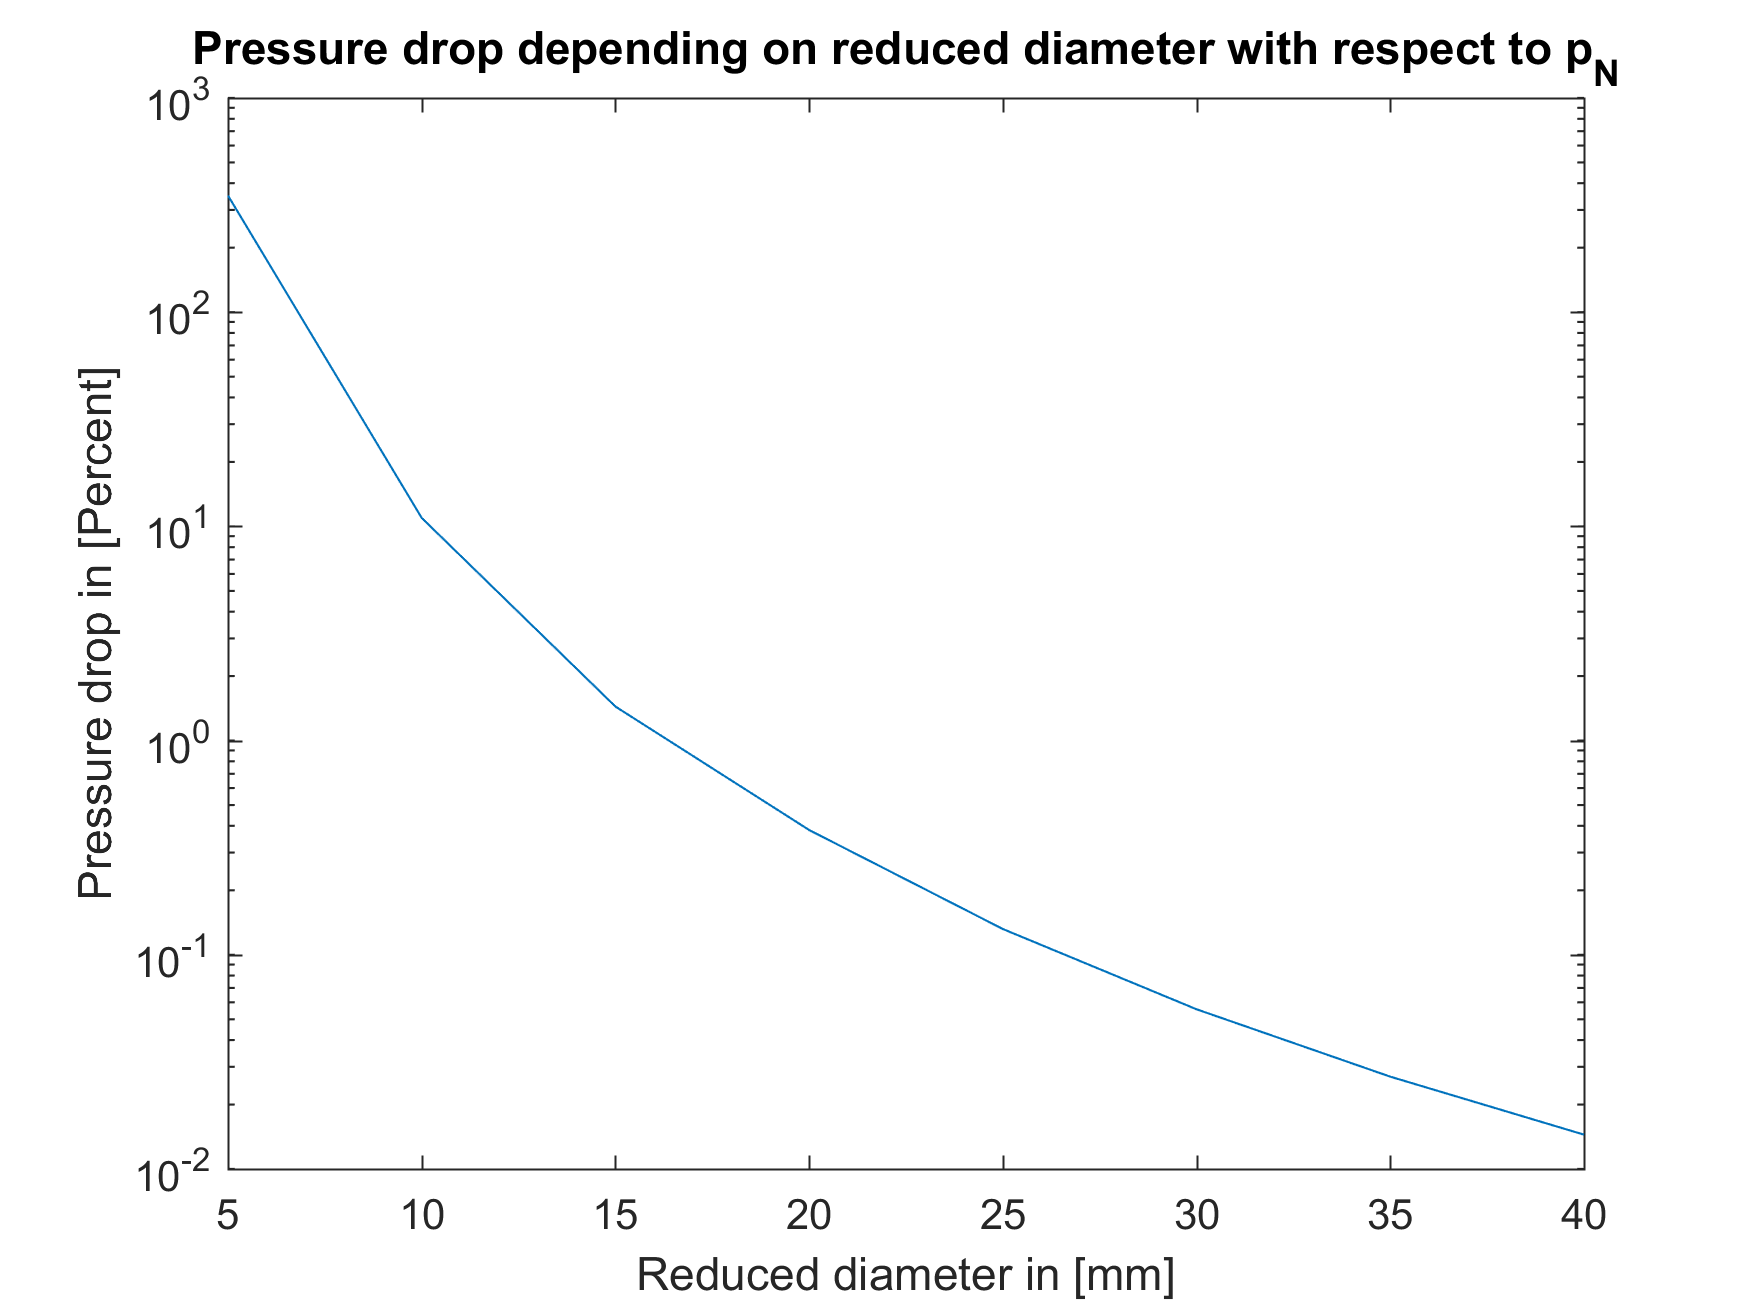
\includegraphics[scale=0.8]{img/PressureDrop}
\caption{}
\label{fig:PressureDrop}
\end{figure}

\vfill

Grundlagen der Fehlerberechnung: 

\url{http://ipl.physics.harvard.edu/wp-uploads/2013/03/PS3_Error_Propagation_sp13.pdf}








\end{document}
